\documentclass{amsart}


\usepackage[utf8]{inputenc}
\usepackage{color}
\usepackage{mathrsfs}
\usepackage{hyperref}
\usepackage{tikz-cd}
\usepackage{mathtools}
\usepackage{csquotes}
\usepackage{tikz}
\usepackage{enumerate}
\usetikzlibrary{arrows}

\newcommand{\ds}[1]{\ensuremath{ \displaystyle{#1} }}

\title{Shor's algorithm}
\author{Jacob Hegna}
\date{\today}

\newcommand{\Zz}{\mathbb{Z}}
\newcommand{\Gg}{\mathbb{G}}
\newcommand{\Hh}{\mathbb{H}}
\newcommand{\Top}{\mathbf{Top}}
\newcommand{\Sch}{\mathbf{Sch}}
\DeclareMathOperator{\per}{per}
\DeclareMathOperator{\lcd}{lcd}
\DeclareMathOperator{\Ab}{Ab}
\DeclareMathOperator{\Cov}{Cov}
\DeclareMathOperator{\Cl}{Cl}
\DeclareMathOperator{\St}{St}
\DeclareMathOperator{\link}{link}
\DeclareMathOperator{\Sub}{Sub}
\DeclareMathOperator{\Spec}{Spec}
\DeclareMathOperator{\Ann}{Ann}
\DeclareMathOperator{\Mod}{Mod}
\DeclareMathOperator{\mmod}{mod}
\DeclareMathOperator{\coker}{coker}
\DeclareMathOperator{\Comm}{Comm}
\DeclareMathOperator{\conv}{conv}
\DeclareMathOperator{\diag}{diag}
\DeclareMathOperator{\Ext}{Ext}
\DeclareMathOperator{\Tor}{Tor}
\DeclareMathOperator{\Gr}{Gr}
\DeclareMathOperator{\Hom}{Hom}
\DeclareMathOperator{\im}{im}

\newtheorem{theorem}{Theorem}[section]
\newtheorem{proposition}[theorem]{Proposition}
\newtheorem{lemma}[theorem]{Lemma}
\newtheorem{corollary}[theorem]{Corollary}
\theoremstyle{definition}
\newtheorem{definition}[theorem]{Definition}
\newtheorem{example}[theorem]{Example}
\newtheorem{remark}[theorem]{Remark}
\theoremstyle{remark}

\newcommand{\abs}[1] {
  \left| #1 \right|}

\newcommand{\norm}[1] {
  \left| \abs{#1} \right|}

\newcommand\restr[2]{{% we make the whole thing an ordinary symbol
  \left.\kern-\nulldelimiterspace % automatically resize the bar with \right
  #1 % the function
  \vphantom{|} % pretend it's a little taller at normal size
  \right|_{#2} % this is the delimiter
  }}

\newcommand{\ket}[1] {|#1\rangle}
\newcommand{\bra}[1] {\langle#1|}
\newcommand{\braket}[2] {\langle#1|#2\rangle}

\begin{document}

\maketitle

\begin{abstract}
    We give a short exposition of Shor's algorithm, which decides primality in
    polynomial time on a quantum computer. We utilize a standard exposition
    found in the literature which exports a bulk of the work to a quantum
    Fourier transform.
\end{abstract}

\tableofcontents

\section{Introduction}

It is a famous theorem that given an integer $n \in \Zz$, there is a unique
expression
\[
    n = \alpha \prod_{i = 0}^k p_i,
    \quad p_i \text{ prime for all } i,
    \quad \alpha \in \Zz^\times.
\]
In fact, this property is one of the most desirable properties that an algebra
can have. Many other algebraic properties (locality, regularity, depth, etc) are
a way to measure how close the structure is to achieving unique factorization.
One could argue that the entire field of number theory is based on this simple
fact.

This result is also fundamental to modern cryptography. The exact details are
out of the scope of this expository note, but it is conjectured that the problem
of prime factorization cannot be solved in polynomial time on a classical
computer. Clearly, however, given $n$ and a collection of primes $\{p_i\}$, one
can verify with $\mathcal{O}(n^3)$ steps that $n = \pm \prod p_i$.

The situation is slightly different with quantum circuits.

\begin{theorem}[Peter Shor]
    Supposing access to quantum circuits, primality is decidable in polynomial
    time.
\end{theorem}

The proof requires a reduction via classical methods, an analysis of an
eigenvalue problem, then concludes with a standard phase estimation circuit
common in quantum computing.

\section{The classical reduction}

Throughout, let $y \in \Zz$ be fixed. We compute the predicate
\[
    \psi(y) = \begin{cases}
        0 \quad \text{if $y$ is prime,} \\
        1 \quad \text{else.}
    \end{cases}.
\]
As it imposes no additional complexity, our algorithm will additionally return a
single prime divisor $p$ of $y$ if $\psi(y) = 1$. Before giving the algorithm,
we refresh the reader on an important definition.

\begin{definition}
    Given a group $\mathbb{G}$ written multiplicatively and an element $g \in
    G$, the \textit{period} of $g$ is the integer $\min \{ n \in \Zz_{> 1} \mid
    g^n = 1_\mathbb{G} \}$. If $\mathbb{G} = \Zz_q$, we use the notation
    $\per_q(g)$ for the period of $g$ in $\mathbb{G}$.
\end{definition}

\subsection{The algorithm}

This classical procedure is taken quite directly from \cite{textbook}. The input
is an integer $y \in \Zz_{> 1}$. The output is a pair $(\alpha, \beta)$ where
$\alpha = \psi(y)$ and $\beta$ is a (not necessarily prime) divisor of $y$ if
$\alpha = 1$.

\textit{Step 1.} Return $(1, 2)$ if $y \equiv 0 \mod 2$. Else, continue.

\textit{Step 2.} Check if $y = m^k$ for $m \in \{2, \dots, \log_2{y}\}$. If so,
return $(1, m)$. Else, continue.

\textit{Step 3.} Impose a uniform distribution on the set $\{0, \dots, y - 1\}$
and sample it for an integer $a$. If $\gcd(a, y) = b > 1$, return $(1, b)$.
Else, continue with $a$ reserved.

\textit{Step 4.} Compute $r = \per_y(a)$ using quantum methods. If $r$ is odd,
output $(0, 0)$. Else, continue with $r, a$ reserved.

\textit{Step 5.} Compute $d = \gcd(a^{r/2} - 1, y)$. If $d > 1$, return $(1,
d)$. Else, return $(0, 0)$.

We have the following lemmas from \cite{textbook} which verify correctness of
the algorithm.

\begin{lemma}
    If the given algorithm returns $(1, d)$, then $d$ is a nontrivial divisor of
    the input. However, if the algorithm returns $(0, s)$ for some $s$, it is
    not necessarily true that the input is prime.
\end{lemma}

\begin{proof}
    Omitted.
\end{proof}

\begin{lemma}
    The probability that the algorithm is correct for a given input $y$ with $k$
    distinct prime divisors is at least $1 - 1/2^{k-1}$.
\end{lemma}

\begin{proof}
    Omitted.
\end{proof}

\section{Determining the period}

To determine the period, we begin by noting that the map
\[
    x \mapsto a^x \mod q,
\]
for $a$, $q$ coprime is a permutation of the integers $\{0, 1, \dots, q\}$. The
orbit of this action which contains $1$ is precisely size $\per_q(a)$ (this is a
rephrasing of the definition). So, given some encoding of an integer $x$ on $n$
bits (so that $q \leq 2^n$), we define a function $f$ which maps $x$ to $a^x \mod
q$ if $x \leq q$ and to $x$ otherwise. $f$ is a permutation on $n$ bits, so we
may consider the operator $U_a := \widehat{f}$. We have the following lemma,
taken from \cite{hw012}.

\begin{lemma}
    $\displaystyle \ket{\xi_k} =
    \frac{1}{\sqrt{t}}\sum_{m=0}^{t-1} e^{-2 \pi i (km/t)} \ket{a^m}$ is an
    eigenvector of $U_a$ with eigenvalue $\lambda_k = e^{2\pi i (k/t)}$.
\end{lemma}

\begin{proof}
    The operator $U_a$ induces a permutation on the set of vectors $\{\ket{1},
    \ket{a^1}, \ket{a^2}, \dots, \ket{a^t}\}$ which maps $\ket{a^\ell}$ to
    $\ket{a^{\ell+1}}$, where addition in the exponent is interpreted modulo
    $t$.  For $\ell \neq t-1$, we have that the $\ell + 1$'th summand in
    $\ket{\xi_k}$ is equal to $e^{2\pi i(k/t)}$ times the $\ell$th summand.  For
    the exceptional case $\ell = t-1$, one must observe that $e^{-2\pi i (t -
        1)k/t} = e^{2\pi i k/t}$ (the exponent in the first expression
    distributes into $-2\pi i k + 2\pi i k/t$, which is the same rotation as the
    second expression).
\end{proof}

Indeed, the $t$ in the expansion of the eigenvalue $\lambda_k$ is precisely
$\per_q(a)$. Thus, if we can estimate this value with a probability bounded
above $1/2$, we are done. Unfortunately, given an eigenvalue $\lambda_k$, we
only know the value $k/t$, which may be reduced if $\gcd(k, t) > 1$. However,
this problem will be resolved later.

\section{Quantum Fourier Transform}

We digress to implement a necessary circuit efficiently. We follow the
exposition in \cite{qft}.

\begin{definition}
    The \textit{Quantum Fourier Transform} is the unitary operation which maps a
    pure state $\ket{x}$ on $2^n$ qubits to
    \[
        \frac{1}{2^{n/2}} \sum_{k=1}^{2^n - 1} \omega^{x k} \ket{k},
    \]
    where $\omega$ is a $2^n$th root of unity. It is defined for mixed states by
    linearity.
\end{definition}

To write an efficient circuit for $\mathit{QFT}$, we need the following fact.

\begin{theorem}
    Let $\ket{x}$ be a pure state. Let $(0.x_1x_2 \dots x_n) = x_1 2^{-1} + x_2
    2^{-2} + \cdots + x_n 2^{-n}$ be the binary decimal. Then,
    \[
        \mathit{QFT}(\ket{x}) = \frac{1}{2^{n/2}} \bigotimes_{r=1}^{n} \left(
            \ket{0} + e^{-2 \pi i x 2^{-r}} \ket{1}
        \right).
    \]
\end{theorem}

\begin{proof}
    The proof is a direct calculation.
    \begin{align*}
        \sum_{k=1}^{2^n - 1} \omega^{x k} \ket{k}
        &= \sum_{k_1, \dots, k_n \in \{0, 1\}} \omega^{-x \sum_{r=1}^n 2^{n-r}
            k_r} \ket{k_1} \otimes \dots \otimes \ket{k_n} \\
        &= \sum_{k_1, \dots, k_n \in \{0, 1\}} \bigotimes_{r=1}^n \omega^{-x
            2^{n-r}} \ket{k_r} \\
        &= \bigotimes_{r=1}^n \left( \sum_{k_r \in \{0, 1\}} \omega^{-x
                2^{n-r}k_r } \ket{k_r}\right)
        \intertext{At this point, note that we are summing over two values and
            we can just expand the sum.}
        &= \bigotimes_{r=1}^n \left( \ket{0} + \omega^{-x 2^{n-r}}
            \ket{1}\right) \\
        &= \bigotimes_{r=1}^n \left( \ket{0} + e^{-2 \pi i x 2^{-r}}\ket{1}
        \right)
    \end{align*}
    We now compute the exponent of the root of unity.
    \[
        -2 \pi i \sum_{\ell = 1}^n 2^{n - r - \ell} x_\ell
        = -2 \pi i (0.x_{n - r + 1} x_{n - 2 + 2} \dots x_n).
    \]
    Multiply everything by $\frac{1}{2^{n/2}}$ and the proof is complete.
\end{proof}

We want to operate on qubits by multiplying their $\ket{1}$th coordinate by
$e^{-2 \pi i 2^{-s}}$ if $x_s = 1$, while fixing the $\ket{0}$th coordinate. By
the magic of linear algebra, let us define
\[
    R_n :=
    \begin{pmatrix}
        1 & 0 \\
        0 & e^{-2 \pi i 2^{-s}}
    \end{pmatrix}.
\]
It is unitary by inspection (othonormal columns). Note that in the expression of
the $\mathit{QFT}$ from the prior problem, the value of the $j$th coordinate
qubit in the original state only affects the value of the $i$th coordinate of
the new state if $i \leq j$. With these two observations, we give the following
circuit.

\begin{center}
    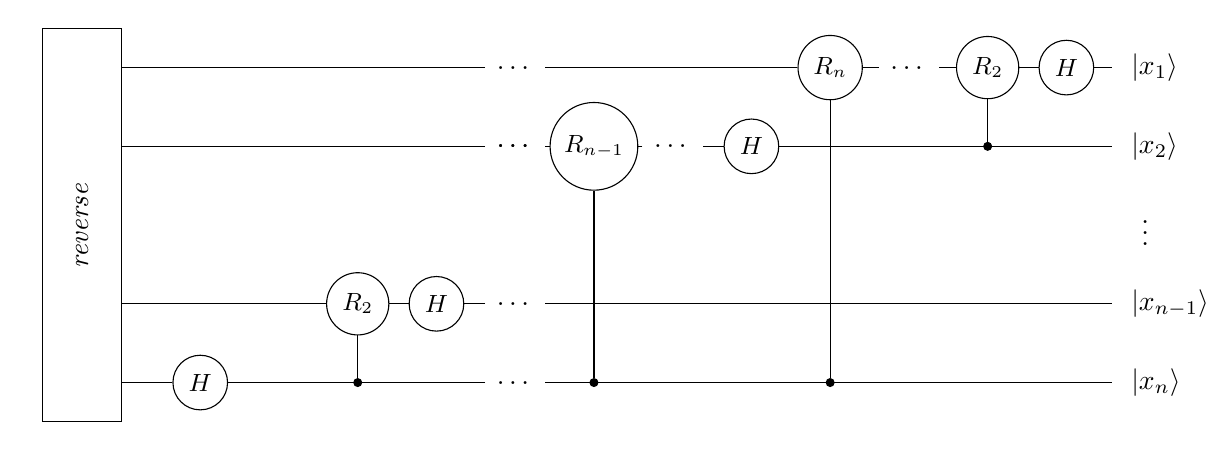
\begin{tikzpicture}
        \tikzset{qubit/.style = {shape=circle,minimum size=2em, text
                width=1em}}
        \tikzset{gate/.style = {shape=circle,draw, font=\small}}
        \tikzset{dot/.style = {shape=circle,fill=black,draw,scale=0.3}}
        \tikzset{dots/.style = {shape=circle,minimum size=1em}}
        \tikzset{edge/.style = {-}}

        \node[qubit] (x1) at (4, 2) {$\ket{x_1}$};
        \node[qubit] (x2) at (4, 1) {$\ket{x_2}$};
        \node[dots] (d) at (4, 0) {$\vdots$};
        \node[qubit] (x3) at (4, -1) {$\ket{x_{n-1}}$};
        \node[qubit] (x4) at (4, -2) {$\ket{x_n}$};

        \node[dots] (d1) at (-4, 2) {$\dots$};
        \node[gate] (H1) at (3, 2) {$H$};
        \node[gate] (R11) at (2, 2) {$R_2$};
        \node[dots] (d0) at (1, 2) {$\dots$};
        \node[gate] (R12) at (0, 2) {$R_n$};

        \node[dots] (H3) at (-4, 1) {$\dots$};
        \node[gate] (H2) at (-1, 1) {$H$};
        \node[dots] (d2) at (-2, 1) {$\dots$};
        \node[dots] (d22) at (-4, 1) {$\dots$};
        \node[gate] (R2) at (-3, 1) {$R_{n-1}$};

        \node[dots] (d3) at (-4, -1) {$\dots$};
        \node[gate] (H3) at (-5, -1) {$H$};
        \node[gate] (R3) at (-6, -1) {$R_2$};

        \node[dots] (d4) at (-4, -2) {$\dots$};
        \node[gate] (H4) at (-8, -2) {$H$};

        \draw[edge] (x1) to (H1);
        \draw[edge] (x2) to (H2);
        \draw[edge] (x3) to (d3);
        \draw[edge] (d3) to (H3);
        \draw[edge] (x4) to (d4);
        \draw[edge] (d4) to (H4);

        \draw[edge] (H1) to (R11);
        \draw[edge] (R11) to (d0);
        \draw[edge] (d0) to (R12);
        \draw[edge] (R12) to (d1);
        \draw[edge] (d1) to (-9, 2);

        \draw[edge] (H2) to (d2);
        \draw[edge] (d2) to (R2);
        \draw[edge] (R2) to (d22);
        \draw[edge] (d22) to (-9, 1);

        \draw[edge] (H3) to (R3);
        \draw[edge] (R3) to (-9, -1);

        \draw[edge] (H4) to (-9, -2);

        \node[dot] (R11c) at (2, 1) {};
        \draw[edge] (R11c) to (R11);
        \node[dot] (R12c) at (0, -2) {};
        \draw[edge] (R12c) to (R12);

        \node[dot] (R2c) at (-3, -2) {};
        \draw[edge] (R2c) to (R2);

        \node[dot] (R3c) at (-6, -2) {};
        \draw[edge] (R3c) to (R3);

        \node[dots, rotate=90] (asdf) at (-9.5, 0) {$\mathit{reverse}$};
        \draw[draw=black] (-10, 2.5) rectangle ++(1, -5);
    \end{tikzpicture}
\end{center}

\begin{proposition}
    The circuit computes $\mathit{QFT}(\ket{x})$ for a pure state $\ket{x}$.
\end{proposition}

\begin{proof}
    For the $i$th qubit in $\ket{x}$, the circuit prior to the reverse gate
    gives
    \[
        \frac{1}{\sqrt{2}} \left( \ket{0} + e^{2\pi i (0.j_i j_{i+1} \dots
                j_{n})}\right)
    \]
    by definition of $\Lambda(R_n)$. This is the value we wish to have in the
    $n-i$th qubit. Thus, after application of the reverse gate, the circuit is
    correct.
\end{proof}

\begin{proposition}
    $\mathit{QFT}$ is unitary, as it is representable by a quantum circuit.
\end{proposition}

\begin{theorem}
    $\mathit{QFT}$ and $\mathit{QFT}^{-1}$ are computable with
    $\mathcal{O}(n^2)$ quantum gates.
\end{theorem}

\begin{proof}
    Proving the theorem for $\mathit{QFT}$ proves it for $\mathit{QFT}^{-1}$
    automatically (they require the same number of gates). There are $n(n+1)/2$
    gates before the reverse circuit, which contains the floor of $n/2$ gates of
    its own.
\end{proof}

\section{Phase estimation}

Currently the goal, more generally, is to compute $\phi$ where $U \ket{\psi} =
e^{2 \pi i \phi} \ket{\psi}$ (an eigenvalue problem).

Begin with an $n$-qubit register initialized to $0$, and an $n$-qubit register
initialized to the encoding of $\psi$, so we have the
state $\ket{0^n} \otimes \ket{\psi}$. We apply the $n$-qubit Hadamard gate
$H^{\otimes n}$ to the first register, and have the $i$th qubit of the first
register control the operator $U^{2^i}$ on the second register.
Diagrammatically,

\begin{center}
    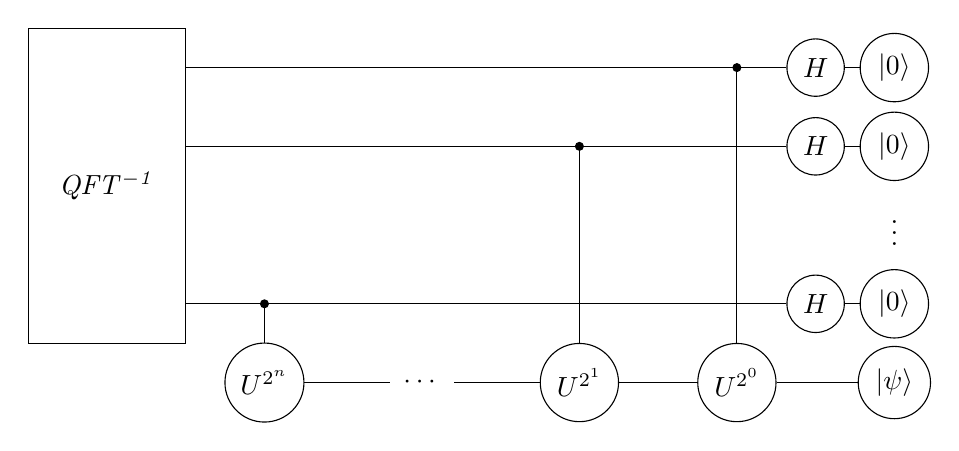
\begin{tikzpicture}
        \tikzset{qubit/.style = {shape=circle,draw,minimum size=1em}}
        \tikzset{dot/.style = {shape=circle,fill=black,draw,scale=0.3}}
        \tikzset{dots/.style = {shape=circle,minimum size=1em}}
        \tikzset{edge/.style = {-}}

        \node[qubit] (R1) at (4, 2) {$\ket{0}$};
        \node[qubit] (R2) at (4, 1) {$\ket{0}$};
        \node[dots] (R3) at (4, 0) {$\vdots$};
        \node[qubit] (R4) at (4, -1) {$\ket{0}$};
        \node[qubit] (R5) at (4, -2) {$\ket{\psi}$};

        \node[qubit] (H1) at (3, 2) {$H$};
        \node[qubit] (H2) at (3, 1) {$H$};
        \node[qubit] (H4) at (3, -1) {$H$};


        \node[dot] (R1U) at (2, 2) {};
        \node[dot] (R2U) at (0, 1) {};
        \node[dot] (R4U) at (-4, -1) {};

        \node[qubit] (U1) at (2, -2) {$U^{2^0}$};
        \node[qubit] (U2) at (0, -2) {$U^{2^1}$};
        \node[dots] (U3) at (-2, -2) {$\cdots$};
        \node[qubit] (U4) at (-4, -2) {$U^{2^n}$};

        \draw[edge] (U1) to (U2);
        \draw[edge] (U2) to (U3);
        \draw[edge] (U3) to (U4);

        \draw[edge] (R5) to (U1);
        \draw[edge] (R1) to (H1);
        \draw[edge] (R2) to (H2);
        \draw[edge] (R4) to (H4);

        \draw[edge] (H1) to (-5, 2);
        \draw[edge] (H2) to (-5, 1);
        \draw[edge] (H4) to (-5, -1);


        \draw[edge] (R1U) to (U1);
        \draw[edge] (R2U) to (U2);
        \draw[edge] (R4U) to (U4);

        \node[dots] (QFT) at (-6, 0.5) {$\mathit{QFT^{-1}}$};
        \draw[draw=black] (-7, 2.5) rectangle ++(2, -4);
    \end{tikzpicture}
\end{center}

This circuit has $\mathcal{O}(n^2)$ gates for the inverse Quantum Fourier
transform, and (when only given $U := U_a$), $\sum_{k=1}^n 2^k + n \leq n^3 + n$
gates for the rest of the circuit. This gives a total complexity of
$\mathcal{O}(n^3)$ gates.

Now, let's compute the state in the first register before the inverse quantum
Fourier transform. Trivially, we have that the state is
\[
    \frac{1}{2^{n/2}} \sum_{k = 0}^{2^n - 1} \ket{k} U^k \ket{\psi}.
\]
However, we know that $U^k \ket{\phi} = e^{2 \pi k i \phi} \ket{\psi}$, so the
state is indeed
\[
    \frac{1}{2^{n/2}} \sum_{k = 0}^{2^n - 1} e^{2 \pi k i \phi} \ket{k}
        \ket{\psi}.
\]

This is precisely the quantum Fourier transform of $\ket{\phi} \otimes
\ket{\psi}$!  Now, if we apply the inverse quantum Fourier transform and measure
the first register, we will measure state $\phi$.

Unfortunately, the eigenvalues of $U_a$ themselves encode the period we desire.
Fortunately, we have the following lemma from \cite{hw012}.

\begin{lemma}
    The sum of the eigenvectors $\xi_k$ of $U_a$ are equal to $\ket{1}$.
\end{lemma}

\begin{proof}
    Consider the coefficients of the vector on the right hand side of the
    following:
    \[
        \ket{1} = \frac{1}{\sqrt{t}} \sum_{k=0}^{t-1} \ket{\xi_k}.
    \]
    Each coefficient is of the form
    \[
        \frac{1}{t} \sum_{k=0}^{t-1} e^{-2\pi i (km /t)},
    \]
    for some $m$. In the case $m = 0$, we clearly have the coefficient is $1$.
    To analyze the case $m > 1$, we recall from problem $2$ that $e^{-2\pi i
        (m/t)}$ satisfies $x^t - 1 = 0$. Thus, it satisfies either $x-1=0$
    or $\sum_{k=0}^{t-1} x^k = 0$ (one can see geometrically that it must be the
    second). However, this implies all the coordinates outside of the
    $\ket{1}$th are zero.
\end{proof}

Thus, if we use $\ket{\phi} = \ket{1}$, we will sample a uniform distribution
over $km/t$ for $k \in \{0, \dots, t-1\}$. There are now two ways to recover
$t$. The first is involves continued fractions.

\subsection{Estimating $t$ with continued fractions}

We cite the following results from the literature. For a reference, see
\cite{math}.

\begin{theorem}
    Let $x \in \mathbb{Q}$. Let $s, r \neq 0$ be two integers. If
    \[
        \abs{x - \frac{s}{r}} < \frac{1}{2 r^2},
    \]
    then $s/r$ is a convergent of $x$.
\end{theorem}

\begin{theorem}
    Let $c := km/t$ as the measurement of the previous quantum circuit. Then,
    the probability that there exists an integer $s$ so that $\gcd(s, t) = 0$
    and
    \[
        \abs{\frac{c}{2^n} - \frac{s}{r}} < \frac{1}{2r^2}
    \]
    is bounded below by
    \[
        \frac{4}{\pi^2} \frac{\phi(t)}{t} \left( 1 - \frac{1}{N} \right)
    \]
    where $\phi(t)$ is Euler's totient function.
\end{theorem}

Now, with these two results, we may end the proof of the algorithm. There exists
(with bounded probability) a measurement of the first quantum register $c$ such
that $\abs{c/2^n - s/t} < \frac{1}{2t^2}$ for $t$ the period and $\gcd(s, t) =
1$. We compute (in polynomial time) the value $s$ for the expansion of $c/2^n$
(this is just Euler's algorithm), then simply check if the denominator of
$\frac{s}{t}$ (by hypothesis this is reduced) is $\per_q(a)$.

\subsection{Estimating $t$ by $\lcd$ methods}

\begin{proposition}
    Given $\ell > 2$ fractions of the form $k_i/t$ written in their reduced form
    as $k_i'/t_i'$, the probability that their least common denominator is not
    $t$ is less than $3 \cdot 2^{-\ell}$.
\end{proposition}

\begin{proof}
    The problem is equivalent to determining the probability that $\gcd(k_1, \dots,
    k_\ell)$ is greater than $1$. Given a fixed prime $p$, the probability that
    $p$ divides each $k$ is bounded above by $1/p^\ell$. To compute the
    probability that the $k_i$'s have a common divisor greater than $1$, we must
    sum the prior estimate for all primes $p$, so we have
    \[
        \sum_{\text{$p$ prime}} \frac{1}{p^\ell} < \sum_{k = 1}^{\infty}
        \frac{1}{k^\ell} < 3 \cdot 2^{\ell},
    \]
    computed as a geometric series.
\end{proof}

We many compute the $\lcd$ in $\mathcal{O}(n^3)$ steps, giving $t$.

\bibliography{bibliography}
\bibliographystyle{ieeetr}

\end{document}
